%%%%%%%%%%%%%%%%%%%%%%%%%%%%%%%%%%%%%%%%%%%%%%%%%%%%%%%%%%%%%%%%%%%%%%%%%%%%%%%%%%
\begin{frame}[fragile]\frametitle{}
\begin{center}
{\Large Data Exploration - Olympics}
\end{center}

{\tiny (Ref: mlcourse.ai Assignment 1 – Open Machine Learning Course)}
\end{frame}

%%%%%%%%%%%%%%%%%%%%%%%%%%%%%%%%%%%%%%%%%%%%%%%%%%%%%%%%%%
\begin{frame}[fragile]\frametitle{Read Data}	
Download the file athlete\_events.csv from Kaggle page. 
https://www.kaggle.com/heesoo37/120-years-of-olympic-history-athletes-and-results

\tiny 
\begin{itemize}
\item ID - Unique number for each athlete
\item Name - Athlete's name
\item Sex - M or F
\item Age - Integer
\item Height - In centimeters
\item Weight - In kilograms
\item Team - Team name
\item NOC - National Olympic Committee 3-letter code
\item Games - Year and season
\item Year - Integer
\item Season - Summer or Winter
\item City - Host city
\item Sport - Sport
\item Event - Event
\item Medal - Gold, Silver, Bronze, or NA
\end{itemize}

\end{frame}

%%%%%%%%%%%%%%%%%%%%%%%%%%%%%%%%%%%%%%%%%%%%%%%%%%%%%%%%%%
\begin{frame}[fragile]\frametitle{Read Data}	
\begin{lstlisting}
import numpy as np
import pandas as pd

PATH = 'athlete_events.csv'
data = pd.read_csv(PATH)
data.head()
\end{lstlisting}

\end{frame}

%%%%%%%%%%%%%%%%%%%%%%%%%%%%%%%%%%%%%%%%%%%%%%%%%%%%%%%%%%
\begin{frame}[fragile]\frametitle{Read Data}	
\begin{center}
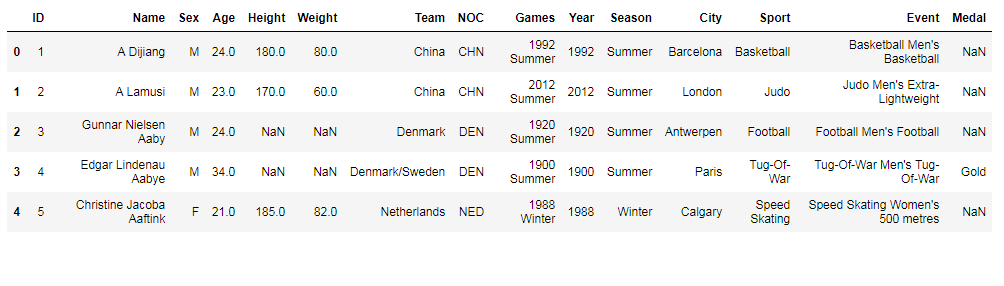
\includegraphics[width=\linewidth,keepaspectratio]{olympics1}
\end{center}
\end{frame}

%%%%%%%%%%%%%%%%%%%%%%%%%%%%%%%%%%%%%%%%%%%%%%%%%%%%%%%%%%
\begin{frame}[fragile]\frametitle{Question 1}	
How old were the youngest male and female participants of the 1996 Olympics?
\begin{itemize}
\item 16 and 15
\item 14 and 12
\item 16 and 12
\item 13 and  11
\end{itemize}

\end{frame}

%%%%%%%%%%%%%%%%%%%%%%%%%%%%%%%%%%%%%%%%%%%%%%%%%%%%%%%%%%
\begin{frame}[fragile]\frametitle{Answer 1}
\begin{lstlisting}
# male
data[(data['Year'] == 1996) & (data['Sex'] == 'M')]['Age'].min()
or
data.loc[(data.Year == 1996) & (data['Sex'] == 'M'), 'Age'].min()
>> 14.0

# female
data[(data['Year'] == 1996) & (data['Sex'] == 'F')]['Age'].min()
or
data.loc[(data.Year == 1996) & (data['Sex'] == 'F'), 'Age'].min()
>> 12.0
\end{lstlisting}

\end{frame}

%%%%%%%%%%%%%%%%%%%%%%%%%%%%%%%%%%%%%%%%%%%%%%%%%%%%%%%%%%
\begin{frame}[fragile]\frametitle{Answer 1}
A "fancier" way:
\begin{lstlisting}
(data[data.Year == 1996]
.groupby('Sex')
.agg('min')
.Age)

>>
Sex
F    12.0
M    14.0
Name: Age, dtype: float64
\end{lstlisting}

\end{frame}



%%%%%%%%%%%%%%%%%%%%%%%%%%%%%%%%%%%%%%%%%%%%%%%%%%%%%%%%%%
\begin{frame}[fragile]\frametitle{Question 2}	
 What was the percentage of male gymnasts among all the male participants of the 2000 Olympics? Round the answer to the first decimal.

Hint: here and further if needed drop duplicated sportsmen to count only unique ones.
\begin{itemize}
\item 0.2
\item 1.5
\item 2.5
\item 7.7
\end{itemize}

\end{frame}

%%%%%%%%%%%%%%%%%%%%%%%%%%%%%%%%%%%%%%%%%%%%%%%%%%%%%%%%%%
\begin{frame}[fragile]\frametitle{Answer 2}
Without dropping duplicates (so, wrong answer)
\begin{lstlisting}
allMale2000 = data[(data['Year'] == 2000) & (data['Sex'] == 'M')].shape[0]
gynastMale2000 = data[(data['Year'] == 2000) & (data['Sex'] == 'M') & (data['Sport'] == 'Gymnastics')].shape[0]
gynastMale2000/allMale2000

>> 0.07651966626936829
\end{lstlisting}

\end{frame}

%%%%%%%%%%%%%%%%%%%%%%%%%%%%%%%%%%%%%%%%%%%%%%%%%%%%%%%%%%
\begin{frame}[fragile]\frametitle{Answer 2}
With dropping duplicates (so, correct answer)
\begin{lstlisting}
q = '(Year == 2000) & (Sex == "M")'
# data.query(q) equals to data[(data.Year == 2000) & (data.Sex == 'M')]
sportsmen_count = len(data.query(q)
                     .drop_duplicates(subset='Name'))
gymnasts_count = len(data.query(q)
                    .query('Sport == "Gymnastics"')
                    .drop_duplicates(subset='Name'))

print('%.1f' % (gymnasts_count / sportsmen_count * 100))

>> 1.5
\end{lstlisting}

\end{frame}

%%%%%%%%%%%%%%%%%%%%%%%%%%%%%%%%%%%%%%%%%%%%%%%%%%%%%%%%%%
\begin{frame}[fragile]\frametitle{Question 3}	
What are the mean and standard deviation of height for female basketball players participated in the 2000 Olympics? Round the answer to the first decimal.
\begin{itemize}
\item 178.5 and 7.2
\item 179.4 and 10
\item 180.7 and 6.7
\item 182.4 and 9.1
\end{itemize}

\end{frame}

%%%%%%%%%%%%%%%%%%%%%%%%%%%%%%%%%%%%%%%%%%%%%%%%%%%%%%%%%%
\begin{frame}[fragile]\frametitle{Answer 3}
\begin{lstlisting}
f2000df = data[(data['Year'] == 2000) & (data['Sex'] == 'F') & (data['Sport'] == 'Basketball')]
f2000df = f2000df.drop_duplicates(keep=False)
f2000df['Height'].mean()

>> 182.38732394366198



f2000df['Height'].std()

>> 9.139462087892174
\end{lstlisting}

\end{frame}

%%%%%%%%%%%%%%%%%%%%%%%%%%%%%%%%%%%%%%%%%%%%%%%%%%%%%%%%%%
\begin{frame}[fragile]\frametitle{Answer 3}
Another way:
\begin{lstlisting}
q = '(Year == 2000) & (Sex == "F") & (Sport == "Basketball")'
(data.query(q)
.describe()
.Height)

>> 
count    142.000000
mean     182.387324
std        9.139462
min      162.000000
25%      175.000000
50%      182.000000
75%      190.000000
max      213.000000
Name: Height, dtype: float64
\end{lstlisting}

\end{frame}

%%%%%%%%%%%%%%%%%%%%%%%%%%%%%%%%%%%%%%%%%%%%%%%%%%%%%%%%%%
\begin{frame}[fragile]\frametitle{Question 4}	
Find a sports-person participated in the 2002 Olympics, with the highest weight among other participants of the same Olympics. What sport did he or she do?
\begin{itemize}
\item Judo
\item Bobsleigh
\item Weightlifting
\item Boxing
\end{itemize}

\end{frame}

%%%%%%%%%%%%%%%%%%%%%%%%%%%%%%%%%%%%%%%%%%%%%%%%%%%%%%%%%%
\begin{frame}[fragile]\frametitle{Answer 4}
\begin{lstlisting}
data.loc[data[(data['Year'] == 2002)]['Weight'].argmax(),'Name']

>> 'Emmanuel Hostache'

data.loc[data[(data['Year'] == 2002)]['Weight'].argmax(),'Sport']

>> 'Bobsleigh'
\end{lstlisting}

\end{frame}

%%%%%%%%%%%%%%%%%%%%%%%%%%%%%%%%%%%%%%%%%%%%%%%%%%%%%%%%%%
\begin{frame}[fragile]\frametitle{Answer 4}
Another way:
\begin{lstlisting}
max_weight_idx = (data[data.Year == 2002]
                 .Weight
                 .idxmax())

(data[data.Year == 2002]
.loc[max_weight_idx]
.Sport)

>> 'Bobsleigh'
\end{lstlisting}

\end{frame}


%%%%%%%%%%%%%%%%%%%%%%%%%%%%%%%%%%%%%%%%%%%%%%%%%%%%%%%%%%
\begin{frame}[fragile]\frametitle{Question 5}	
How many times did Pawe Abratkiewicz participate in the Olympics held in different years?
\begin{itemize}
\item 0
\item 1
\item 2
\item 3
\end{itemize}

\end{frame}

%%%%%%%%%%%%%%%%%%%%%%%%%%%%%%%%%%%%%%%%%%%%%%%%%%%%%%%%%%
\begin{frame}[fragile]\frametitle{Answer 5}
\begin{lstlisting}
data[data['Name'] == 'Pawe Abratkiewicz']['Year'].nunique()

or

len(data[data.Name == 'Pawe Abratkiewicz']
   .drop_duplicates(subset='Year')
   .Year) 

or
len(data[data.Name == 'Pawe Abratkiewicz']
   .groupby('Year'))
   
>> 3
\end{lstlisting}
\end{frame}


%%%%%%%%%%%%%%%%%%%%%%%%%%%%%%%%%%%%%%%%%%%%%%%%%%%%%%%%%%
\begin{frame}[fragile]\frametitle{Question 6}	
How many silver medals in tennis did Australia win at the 2000 Olympics?
\begin{itemize}
\item 0
\item 1
\item 2
\item 3
\end{itemize}

\end{frame}

%%%%%%%%%%%%%%%%%%%%%%%%%%%%%%%%%%%%%%%%%%%%%%%%%%%%%%%%%%
\begin{frame}[fragile]\frametitle{Answer 6}
\begin{lstlisting}
data[(data['Year']==2000) & (data['Team']=='Australia') & (data['Medal']=='Silver') & (data['Sport']=='Tennis')].shape[0]

or
q = '(Year == 2000) & (Team == "Australia") & (Medal == "Silver") & (Sport == "Tennis")'
data.query(q).shape[0]

or
q = '(Year == 2000) & (Team == "Australia")'
(data.query(q)
.groupby(['Medal', 'Sport'])
.get_group(('Silver', 'Tennis'))
.shape[0])
>> 2
\end{lstlisting}

\end{frame}

%%%%%%%%%%%%%%%%%%%%%%%%%%%%%%%%%%%%%%%%%%%%%%%%%%%%%%%%%%
\begin{frame}[fragile]\frametitle{Question 7}	
Is it true that Switzerland won fewer medals than Serbia at the 2016 Olympics? Do not consider NaN values in Medal column?
\begin{itemize}
\item Yes
\item No
\end{itemize}

\end{frame}

%%%%%%%%%%%%%%%%%%%%%%%%%%%%%%%%%%%%%%%%%%%%%%%%%%%%%%%%%%
\begin{frame}[fragile]\frametitle{Answer 7}
\begin{lstlisting}
data[(data['Year']==2016) & (data['Team']=='Switzerland')]['Medal'].dropna().shape[0]
or
Switzerland_medals = len(data.query('(Year == 2016) & (Team == "Switzerland")')
                        .dropna(subset=['Medal']))
>> 11
data[(data['Year']==2016) & (data['Team']=='Serbia')]['Medal'].dropna().shape[0]
or
Serbia_medals = len(data.query('(Year == 2016) & (Team == "Serbia")')
                   .dropna(subset=['Medal']))
>> 54
\end{lstlisting}

\end{frame}

%%%%%%%%%%%%%%%%%%%%%%%%%%%%%%%%%%%%%%%%%%%%%%%%%%%%%%%%%%
\begin{frame}[fragile]\frametitle{Answer 7}
Fancier way:
\begin{lstlisting}
(data[data.Year == 2016]
.dropna(subset=['Medal']) 
.groupby('Team') 
.size()
[['Switzerland', 'Serbia']])

>> 
Team
Switzerland    11
Serbia         54
dtype: int64
\end{lstlisting}

\end{frame}

%%%%%%%%%%%%%%%%%%%%%%%%%%%%%%%%%%%%%%%%%%%%%%%%%%%%%%%%%%
\begin{frame}[fragile]\frametitle{Question 8}	
What age category did the fewest and the most participants of the 2014 Olympics belong to?
\begin{itemize}
\item [45-55] and [25-35) correspondingly
\item [45-55] and [15-25) correspondingly
\item [35-45] and [25-35) correspondingly
\item [45-55] and [35-45) correspondingly
\end{itemize}

\end{frame}

%%%%%%%%%%%%%%%%%%%%%%%%%%%%%%%%%%%%%%%%%%%%%%%%%%%%%%%%%%
\begin{frame}[fragile]\frametitle{Answer 8}
\begin{lstlisting}
ranges = [5,15,25,35,45,55]
pd.cut(data[(data['Year']==2014)]['Age'], ranges).value_counts().head(1)

>> (15, 25]    2412

pd.cut(data[(data['Year']==2014)]['Age'], ranges).value_counts().tail(1)

>> (45, 55]    4
\end{lstlisting}

Wrong Answer!!
\end{frame}

%%%%%%%%%%%%%%%%%%%%%%%%%%%%%%%%%%%%%%%%%%%%%%%%%%%%%%%%%%
\begin{frame}[fragile]\frametitle{Answer 8}
\begin{lstlisting}
participants_2014 = (data[data.Year == 2014]
                    .drop_duplicates(subset='Name'))
print('[15, 25): ', len(participants_2014.query('(Age >= 15) & (Age < 25)')))
print('[25, 35): ', len(participants_2014.query('(Age >= 25) & (Age < 35)')))
print('[35, 45): ', len(participants_2014.query('(Age >= 35) & (Age < 45)')))
print('[45, 55]: ', len(participants_2014.query('(Age >= 45) & (Age <= 55)')))
>>
[15, 25):  1193
[25, 35):  1396
[35, 45):  150
[45, 55]:  5
\end{lstlisting}
\end{frame}

%%%%%%%%%%%%%%%%%%%%%%%%%%%%%%%%%%%%%%%%%%%%%%%%%%%%%%%%%%
\begin{frame}[fragile]\frametitle{Answer 8}
Fancier way:
\begin{lstlisting}
def age_category(age):
    if 15 <= age < 25:
        return '[15, 25)'
    elif 25 <= age < 35:
        return '[25, 35)'
    elif 35 <= age < 45:
        return '[35, 45)'
    return '[45, 55]'

data['age_category'] = data.Age.map(age_category)
(data[data.Year == 2014]
.drop_duplicates(subset='Name')  
.groupby('age_category')
.size())
>>
age_category
[15, 25)    1193
[25, 35)    1396
[35, 45)     150
[45, 55]       5
dtype: int64
\end{lstlisting}
\end{frame}


%%%%%%%%%%%%%%%%%%%%%%%%%%%%%%%%%%%%%%%%%%%%%%%%%%%%%%%%%%
\begin{frame}[fragile]\frametitle{Question 9}	
Is it true that there were Summer Olympics held in Lake Placid? Is it true that there were Winter Olympics held in Sankt Moritz?
\begin{itemize}
\item Yes, Yes
\item Yes, No
\item No, Yes
\item No, No
\end{itemize}

\end{frame}

%%%%%%%%%%%%%%%%%%%%%%%%%%%%%%%%%%%%%%%%%%%%%%%%%%%%%%%%%%
\begin{frame}[fragile]\frametitle{Answer 9}
\begin{lstlisting}
data[(data['Season']=='Summer') & (data['City']=='Lake Placid')].shape[0]
>> 0
data[(data['Season']=='Winter') & (data['City']=='Sankt Moritz')].shape[0]
>> 1657

or 
(pd.crosstab(data.City, data.Season)
.loc[['Lake Placid', 'Sankt Moritz']])
>>
				Summer	Winter
City		
Lake Placid		0		2098
Sankt Moritz	0		1657
\end{lstlisting}

\end{frame}

%%%%%%%%%%%%%%%%%%%%%%%%%%%%%%%%%%%%%%%%%%%%%%%%%%%%%%%%%%
\begin{frame}[fragile]\frametitle{Question 10}	
What is the absolute difference between the number of unique sports at the 1995 Olympics and 2016 Olympics?
\begin{itemize}
\item 16
\item 24
\item 26
\item 34
\end{itemize}

\end{frame}

%%%%%%%%%%%%%%%%%%%%%%%%%%%%%%%%%%%%%%%%%%%%%%%%%%%%%%%%%%
\begin{frame}[fragile]\frametitle{Answer 10}
\begin{lstlisting}
data[data['Year'] == 1995]['Sport'].nunique()
>> 0
data[data['Year'] == 2016]['Sport'].nunique()
>> 34

or
abs(data[data.Year == 1995].Sport.nunique() - data[data.Year == 2016].Sport.nunique())
\end{lstlisting}

\end{frame}